%!TEX root=../paper.tex

\chapter{Introduction}
\label{sec:intro}

Web technologies have shaped how we think, communicate, and innovate. Over the past decade, the Web's role shifted from solely information retrieval (Web 1.0) to providing interactive user experiences (Web 2.0). Now the Web is once again on the cusp of a new evolution that features automatic recognition, mining, and synthesis of user-originated ``big data.'' The driving force behind this evolution is today's most pervasive personal computing platform---mobile devices. It is estimated that 3~billion Web-connected mobile devices currently exist, and will reach nearly 50~billion by 2020~\cite{Evans:2011ys}. The trend is clear: next-generation Web services will be primarily accessed through mobile devices instead of desktops and laptops as in previous generations~\cite{KPCB-Internet-Trends15}.

While there are significant growth opportunities for mobile Web computing, standing in the way are technology challenges. Specifically, there is a fundamental tension between the ever-increasing computation intensity of Web technologies and the performance and energy-constrained nature of mobile devices. Such a mismatch between computational ``demand and supply'' leads to poor quality-of-service (QoS) experience, resulting in severe consequences. For example, Google estimated that ``a 400~ms delay leads to a 0.44\% drop in search volume.''~\cite{web:google} Similarly, Amazon concluded that a 1-second delay in webpage load time could translate to \$1.6 billion lost in sales annually~\cite{Eaton:2013uq}.

Conventional techniques to improve mobile compute capability have largely been focused on CPU design, largely by adopting desktop-oriented design techniques, i.e., to apply aggressive (micro-)architecture mechanisms for both single-core and multi-core performance while relying the underlying circuit techniques (i.e., Dennard Scaling~\cite{dennard}) for power and energy-efficiency~\cite{mobilecpu}. However, as the demise of the graceful Dennard scaling becomes a reality~\cite{darksilicon}, excessive power and energy consumption will eventually put the CPU-centric, desktop-like design strategy to its end.

\paragraph{Thesis Statement} To sustain mobile performance improvement while being energy-efficient, we must deviate away from the traditional CPU-only mentality. Instead, we must expand the research scope to the entire Web computing stack spanning architecture, runtime, and programming language layers. Following this tenet, my dissertation proposes hardware accelerators, runtime scheduling mechanisms, and programmers-assisted language annotations, the combination of which forms a hardware/software co-designed computing substrate that improves mobile Web performance and energy-efficiency.

The rest of this chapter is organized as follows. \Sect{sec:intro:work} provides an overview of my research contributions. \Sect{sec:intro:impact} discusses the long-term impact of my work. \Sect{sec:intro:scope} puts my work in the broad context of mobile computing. \Sect{sec:intro:outline} outlines the rest of the dissertation and \Sect{sec:intro:prev} lists previously published materials that this dissertation draws upon.

\section{Research Contributions}
\label{sec:intro:work}

The key theme of my work is to deviate away from the general-purpose CPU-centric mindset and to take a holistic view of the mobile Web computation stack spanning application, Web browser runtime, and processor architecture layers. I contend that improving energy-efficiency and performance of mobile Web computing requires us to enhance the traditional computing interfaces with \textit{new abstractions} and to leverage the new interfaces for \textit{cross-layer optimizations}. As such, the central challenge of my research is to carefully forge new abstractions that expose optimization opportunities while enabling effective and practical optimization mechanisms.

At the application/Web browser boundary, current Web applications merely specify visual appearance and functionalities to the browser through Web languages such as HTML, CSS, and JavaScript. User QoS requirements (e.g., latency tolerance) are unexpressed. However, different users QoS requirements lead to different optimal runtime decisions for trading off QoS with energy consumption. Exposing user QoS expectations at the application level would allow the Web runtime to budget wisely the energy usage while delivering satisfactory user QoS experience.

At the Web browser/architecture boundary, the traditional interface provides to the Web browser runtime a simplistic and monolithic execution model of the hardware. However, today's mobile processors are becoming extremely complex, combining general-purpose cores that have different performance and energy characteristics~\cite{single-ISA} with special-purpose domain-specific accelerators. While the hardware upheaval promises performance and energy improvements for the mobile Web, its practical impact depends on how effective the Web browser can leverage it. I see both needs on specializing the processor architecture for the Web domain that enriches the runtime/architecture interface and on designing an intelligent Web browser runtime that can effectively manage the complex interface to optimize for energy-efficiency.

In the spirit of enhancing the traditional Web computing stack interfaces and leveraging the new interfaces to optimize each layer, my dissertation makes the following three contributions. \Fig{fig:framework} provides an overview of the contributions. Enhancements to the existing Web stack are shaded.

\begin{sidewaysfigure}
    \centering
    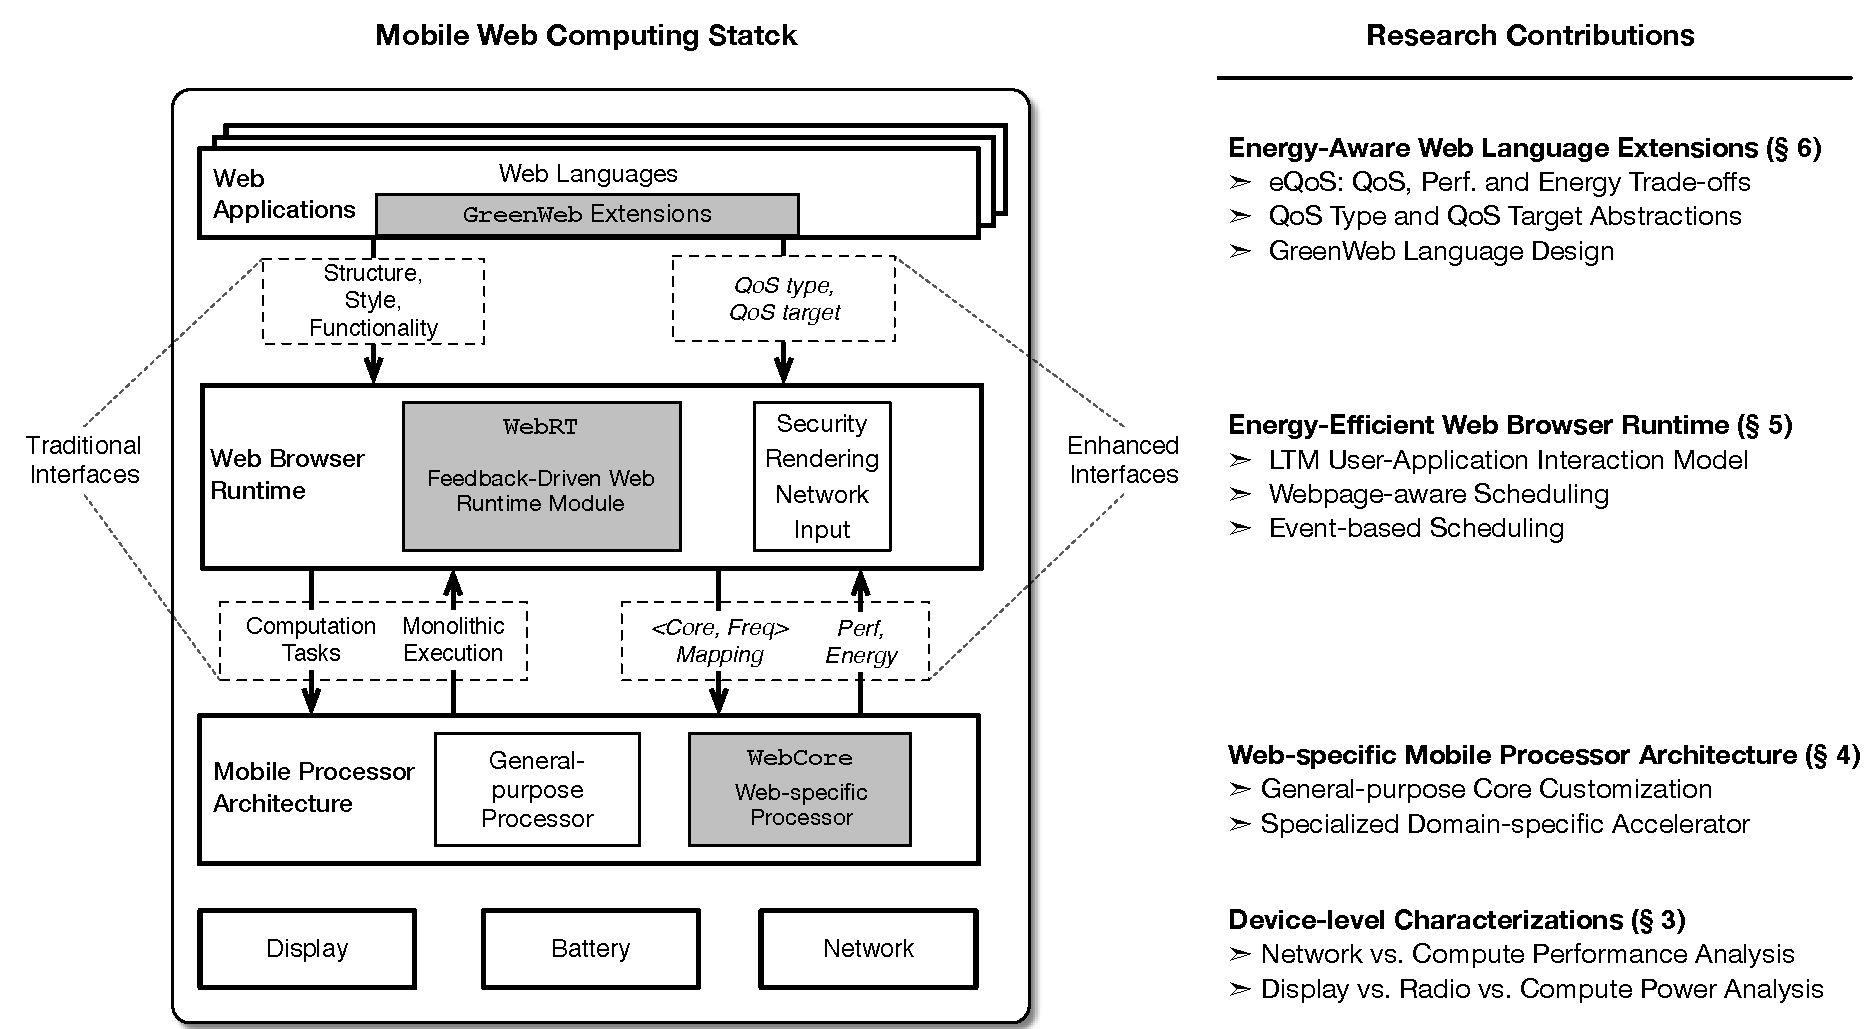
\includegraphics[trim=0 0 0 0, clip, width=1\columnwidth]{framework}
    \caption{Overview of my cross-layer research contributions.}
    \label{fig:framework}
\end{sidewaysfigure}

\begin{itemize}
\item \textbf{Web Language Extensions:} I propose \greenweb, a set of programming language extensions that let Web developers express user QoS expectations as program annotations. \greenweb enhances the traditional application-runtime interface with two new programming abstractions, QoS type and QoS target, that capture two critical aspects of user QoS experience. Exposing QoS requirements in Web applications effectively guides the underlying Web runtime to determine how to deliver the target QoS experience while minimizing the energy consumption. \greenweb does not pose any constraints on specific runtime implementations but instead supports general energy optimization techniques.

\item \textbf{Smart Web Browser Runtime:} I propose \webrt, a  mobile Web browser runtime that optimizes for energy-efficiency while delivering the specified user QoS requirements. Although \webrt is a generic runtime design, I demonstrate a prototype implementation based on the asymmetric chip-multiprocessor (ACMP) hardware architecture. ACMP exposes two new architecture-level abstractions: core type and core frequency. \webrt leverages the new abstractions and dynamically provisions the hardware resources according to user QoS requirements for energy savings. In addition, \webrt also continuously monitors the runtime execution behaviors to enable feedback-driven optimizations, which is critical considering the interactive nature of mobile applications.

\item \textbf{Web-Specific Processor Architecture:} I propose \webcore, a forward-looking mobile CPU architecture customized and specialized for the Web stack. The \webcore improves performance and energy-efficiency simultaneously by integrating domain-specific hardware that exploits critical computation kernels and data communication patterns. A key design goal of \webcore is maintain general-purpose programmability, which is vital to ensure its applicability to the complex Web software stack. Overall, \webcore deepens the heterogeneity of the mobile processor architecture and enlarges the performance-energy trade-off space that the Web runtime can take advantage of.
\end{itemize}

\section{Long-term Impact}
\label{sec:intro:impact}

Mobile hardware and Web software ecosystems undergo rapid design cycles to keep up with constant innovations. It is vital to ensure that any research contributions to this domain have long-term impact, or they perish.

The long-term impact of my work lies in two fundamental aspects. First, the problem that I study is a long-term research agenda. The key challenge that my research focuses on, i.e.,  performance and energy-efficiency, will always be at the forefront of mobile computing research. As the battleground of mobile computing gradually shifts into even smaller form factors such as wearables and Internet-of-Things (IoT) devices, improving performance and energy-efficiency of mobile computing is ever important.

Second, my proposed techniques have long-term applicability because they focus on the fundamental computation layers of Web technologies rather than being tied to the specifics of today's systems. For instance, \webcore proposes a hardware units that optimizes CSS processing, which is a cornerstone technology that remains largely unchanged as new Web standards and specifications come and go. Similarly, the designs of \webrt and \greenweb are also generally applicable because they are do not rely on a particular form of the underlying processor (micro-)architecture or application features.

\section{Research Scope}
\label{sec:intro:scope}

The scope of mobile Web computing is broad and becoming increasingly rich. It involves two critical components: compute and network. The compute component can be further classified by approaches that are either client-centric or based on cloud-offloading. \Fig{fig:scope} shows the hierarchy of the mobile Web scope. My research judiciously focuses on the client-side compute. In other words, it takes a compute-driven and client-centric approach. This section discusses my rational. The goal here is not to dismiss research in network and cloud computing community, but to explain the trade-offs between different approaches and thereby set the context for my work.

\begin{figure}[t]
\centering
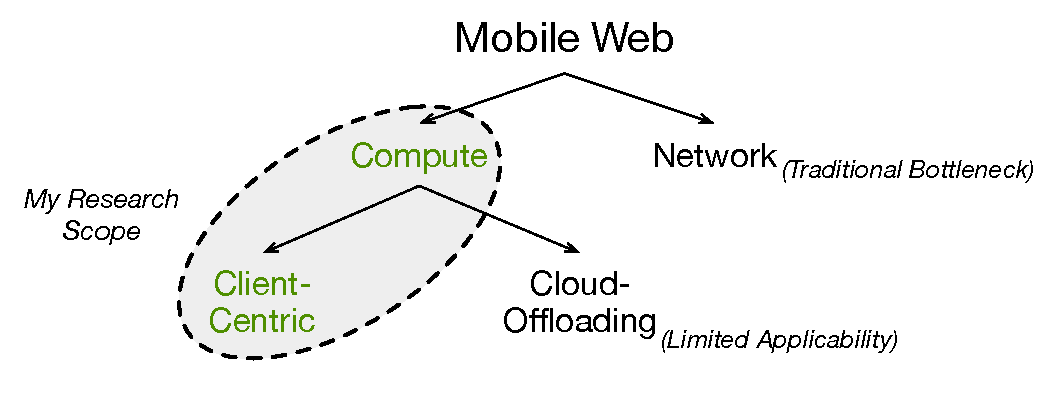
\includegraphics[trim=0 0 0 0, clip, width=.9\columnwidth]{scope}
\caption{The mobile Web computing scope. My research takes a compute-driven, client-centric approach.}
\label{fig:scope}
\end{figure}

\paragraph{Compute-versus-Network} Traditionally when the scope of Web computing was merely about serving static webpages, Web performance was predominantly bottlenecked by network capability because very little processing was involved. However, this trend is changing. Over the past decade cellular network technology has improved dramatically. For example, the round-trip time is improved by two orders of magnitude from 2G to LTE ~\cite{4gtest}. Meanwhile, the computational requirements posed by new Web technologies (e.g., CSS3, HTML5, WebGL) keep increasing. For instance, under the same network condition the processing time for loading the same website from different years over the past decade has increased by as much as 10X~\cite{big-little}. The combined effect of faster network performance and higher computation demand implies that future mobile Web performance will be unattainable without improving the compute capability. An in-depth computer-versus-network bottleneck analysis can be found in \Sect{sec:motivation:perf}.

\paragraph{Client-versus-Cloud} Compute in mobile Web has been primarily carried out by client-side devices only. Recently researcher have started investigating a new compute paradigm where part of the computation is offloaded to cloud platforms through wireless connections---the so called mobile cloud computing (MCC). Although MCC is a promising approach that extends the capability of mobile devices for computation-intensive applications, it has three major limitations. First, today's Web applications are extremely dynamic where both data and code can be generated at runtime depending on user-specific information (e.g., via sensors). The dynamic nature of Web applications leads to frequent synchronizations between client and cloud that potentially undermine the performance and energy-efficiency benefits that MCC brings. Second, MCC assumes the availability of wireless connections, which limits its usage scenario. Third, MCC raises security and privacy concerns as data and computation are transmitted over the network.

The limitations stated above indicate that a handful questions need to be addressed for MCC to succeed. That said, future mobile Web computing systems will most certainly incorporate certain aspects of cloud-offloading, a quantitative trade-off study of which is warranted but beyond my scope.

\section{Dissertation Organization}
\label{sec:intro:outline}

The rest of my dissertation is organized as follows. \Sect{sec:background} introduces the preliminary knowledge of Web computing. \Sect{sec:motivation} quantitatively demonstrates the need for high-performance and energy-efficient computation in the mobile Web, which directly motivates the research theme of my work. \Sect{sec:arch}, \Sect{sec:runtime}, and \Sect{sec:lang} describe the proposed \webcore, \webrt, and \greenweb at the architecture, runtime, and programming language layer, respectively. \Sect{sec:conc} provides a retrospective and prospective view of my dissertation work. The retrospective part summarizes the principles distilled from this work on building a high-performance while energy-efficient mobile Web computing system; the prospective part suggests next steps for generalizing the principles and outlines potential research items for future work.

\section{Previously Published Material}
\label{sec:intro:prev}

This dissertation contains materials that are previously published in peer-reviewed conferences and journals:

\textbf{\Sect{sec:motivation}}. The network-versus-computer analysis in \Sect{sec:motivation:perf} contains results from the following paper: \textit{The Role of the CPU in Energy-Efficient Mobile Web Browsing}. Yuhao Zhu, Matthew Halpern and Vijay Janapa Reddi. In IEEE Micro, Jan/Feb 2015, 35(1):26-33 \cite{zhu2015role}. The power and energy characterizations in \Sect{sec:motivation:energy} contains results from the following paper: \textit{Mobile CPU's Rise to Power: Quantifying the Impact of Generational Mobile CPU Design Trends on Performance, Energy, and User Satisfaction}. Matthew Halpern, Yuhao Zhu and Vijay Janapa Reddi. In High Performance Computer Architecture (HPCA), 2016 \cite{mobilecpu}.

\textbf{\Sect{sec:arch}}. The design and implementation of \webcore are based on the following paper: \textit{WebCore: Architectural Support for Mobile Web Browsing}. Yuhao Zhu and Vijay Janapa Reddi. In International Symposium on Computer Architecture (ISCA), 2014 \cite{webcore}. \Sect{sec:arch} also contains results from the following journal paper: \textit{Optimizing General-Purpose CPUs for Energy-Efficient Mobile Web Computing}. Yuhao Zhu and Vijay Janapa Reddi. In ACM Transactions on Computer Systems (TOCS), March 2017, 35(1):1 \cite{webcore-tocs}.

\textbf{\Sect{sec:runtime}}. The fundamental idea of \webrt is based on the following position paper:  \textit{Exploiting Webpage Characteristics for Energy-Efficient Mobile Web Browsing}. Yuhao Zhu, Aditya Srikanth, Jingwen Leng and Vijay Janapa Reddi. In Computer Architecture Letters (CAL), Oct 2012, 13(1):33-36 \cite{zhu2014exploiting}. The webpage-aware scheduler described in \Sect{sec:runtime:load} draws upon \textit{High-Performance and Energy-Efficient Mobile Web Browsing on Big/Little Systems}. Yuhao Zhu and Vijay Janapa Reddi.  In High Performance Computer Architecture (HPCA), 2013 \cite{big-little}. The event-based scheduler in \Sect{sec:runtime:ebs} draws upon \textit{Event-based Scheduling for Energy-Efficient QoS (eQoS) in Mobile Web Applications}. Yuhao Zhu, Matthew Halpern and Vijay Janapa Reddi. In High Performance Computer Architecture (HPCA), 2015 \cite{ebs}.

\textbf{\Sect{sec:lang}}. The \greenweb language extensions and the \autogreen annotation framework are based on the following paper: \textit{GreenWeb: Language Extensions for QoS-aware Energy-Efficient Mobile Web Computing}. Yuhao Zhu and Vijay Janapa Reddi. In Programming Language Design and Implementation (PLDI), 2016 \cite{greenweb}.


